\begin{figure}%[H]
    \centering
    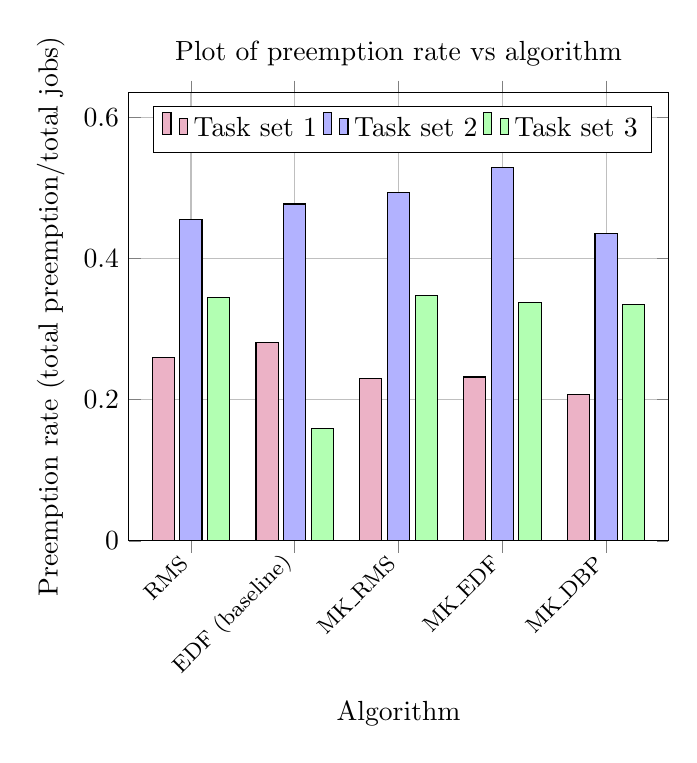
\begin{tikzpicture}
        \begin{axis}[
            ybar,
            title={Plot of preemption rate vs algorithm},
            xlabel={Algorithm},
            ylabel={Preemption rate (total preemption/total jobs)},
            ymin=0.0,
            enlarge y limits={upper, value=0.2},
            grid=major,
            symbolic x coords={RMS, EDF (baseline), MK\_RMS, MK\_EDF, MK\_DBP},
            xtick=data,
            bar width=8pt,
            enlarge x limits=0.15,
            xticklabel style={
                font=\footnotesize,
                rotate=45,
                anchor=east,
            },
            legend style={
                at={(0.97,0.97)},
                anchor=north east,
                legend columns=-1
            },
        ]

        % color1!30!color2, means 30% color1 70% color2
        \addplot+[fill=purple!30!white, draw=black] table [col sep=comma, x=Algorithm, y=prate] {
            Algorithm,prate
            RMS,0.260
            EDF (baseline),0.281
            MK\_RMS,0.230
            MK\_EDF,0.232
            MK\_DBP,0.207
        };\addlegendentry{Task set 1}

        \addplot+[fill=blue!30!white, draw=black] table [col sep=comma, x=Algorithm, y=prate] {
            Algorithm,prate
            RMS,0.455
            EDF (baseline),0.477
            MK\_RMS,0.493
            MK\_EDF,0.529
            MK\_DBP,0.435
        };\addlegendentry{Task set 2}

        \addplot+[fill=green!30!white, draw=black] table [col sep=comma, x=Algorithm, y=prate] {
            Algorithm,prate
            RMS,0.344
            EDF (baseline),0.159
            MK\_RMS,0.347
            MK\_EDF,0.337
            MK\_DBP,0.335
        };\addlegendentry{Task set 3}
        \end{axis}
    \end{tikzpicture}
    \caption{Plot of preemption rate vs algorithm}
    \label{fig:preemption-rate-vs-algo}
\end{figure}